
The distribution of primary papers over time can be seen in Figure~\vref{fig:barchart1} --- papers span from 2007 to 2012 (the mapping study was conducted 2012). Figure~\ref{fig:bubble1} shows a bubble chart of the mapping facets research topic and evaluation method. The totals do not match exactly with the total number of papers included in the study as it is possible for papers to cover both multiple topics and use multiple evaluation methods within the study. This is particularly common where studies use the evaluation approach UP (measuring user performance) as this evaluation method tends to use controlled studies and a corresponding UE (user evaluation) component, such as a lab questionnaire requesting subjective user feedback. It is possible to see in this chart a heavy tendency towards UP and UE evaluation approaches within the domains of text corpora and web. The focus on web and text is not surprising as these are the domains where tag clouds are most commonly found.

\begin{figure}[!htb]
\centering
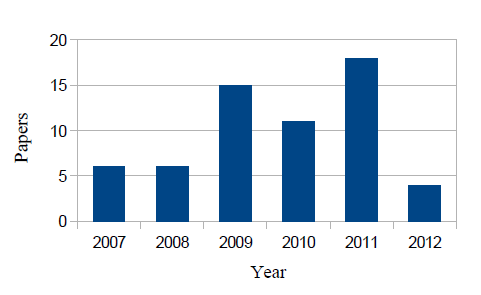
\includegraphics{barchart1.png}
\caption{\textit{Distribution of papers over time}}
\label{fig:barchart1}
\end{figure}

\begin{figure}[!htb]
\centering
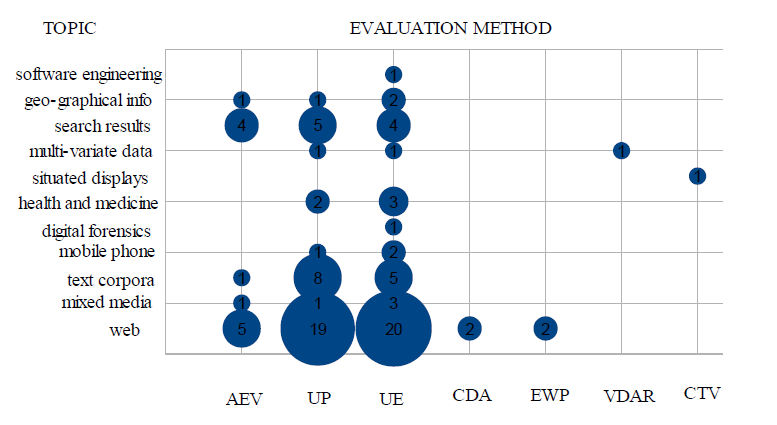
\includegraphics[scale=0.75]{bubble1.png}
\caption{\textit{Mapping facets: research topic and evaluation method}}
\label{fig:bubble1}
\end{figure}

\subsection{Research topic}\label{topic}

A breakdown of the numbers of studies found in each research topic and sub-topic can be found in Table~\vref{tab:researchtopic}. The research topics were heavily skewed towards evaluations of proposed enhancements to tag clouds (see Figure~\vref{fig:pie1}). The most commonly proposed type of enhancement was to cater for a special dataset or medium \citep[such as][]{aras09, kim09, kurtz11, shrinivasan09} where interfaces were built for domains such as geo-graphical information, mobile phone, software engineering or multi-variate data. Other popular topics were proposals for improving perceived tag cloud visualisation shortcomings, such as determining relationships and displaying temporal evolution \citep[for example][]{DiCaro2011120, gomez11}. Only two papers proposed design guidelines or recommendations \citep{rivadeneira07, bateman08}. Evaluations of effectiveness and determining the limits of visual perception made up 22 percent of papers. Tag cloud support was researched by 6 percent of papers for a particular user process.

\begin{landscape}
\begin{table}
\centering
\caption{\textit{Results for the research topic}}
\begin{tabular}{|l|c|p{6cm}|x{2cm}|} \hline
\textbf{Topic}&\textbf{Number}&\textbf{Sub-topic}&\textbf{Number}\\ \hline
Proposal of a tag cloud enhancement&
41&
\parbox[t]{7cm}{\raggedright relationships\break  topic clustering\break temporal evolution\break tag ranking algorithms\break tagging interfaces\break  interface for a special dataset\break interface for a special medium\break layout optimisation}&
7\par 6\par 4\par 9\par 2\par 13\par 2\par 5\\
%relationships\par  topic clustering\par  temporal evolution\par tag ranking algorithms\par tagging interfaces\par  interface for a special dataset\par interface for a special medium\par layout optimisation&7\par 6\par 4\par 9\par 2\par 13\par 2\par 5\\ 
Proposal of evaluation metrics or methodologies&2&&\\
Evaluating the effectiveness of the tag cloud technique&9&&\\
Discovering limits of visual perception&8&visual features or properties\par layout&5\par 3\\
Making design guidelines or recommendations&2&&\\
Determining user motivation for use&3&&\\
Determining support for user process&6&social navigation\par incidental learning\par reflections of learners\par determine credibility of sources\par dynamic representation of places&1\par 1\par 1\par 1\par 1\\
Determining perceived physical demand or workload&2&&\\
Evaluations of systems targeting a special population&4&\par Chinese readers\par Hebrew readers\par tools for the blind&2 \par 1\par 1\par\\
\hline\end{tabular}
\label{tab:researchtopic}
\end{table}
\end{landscape}

\begin{figure}[!htb]
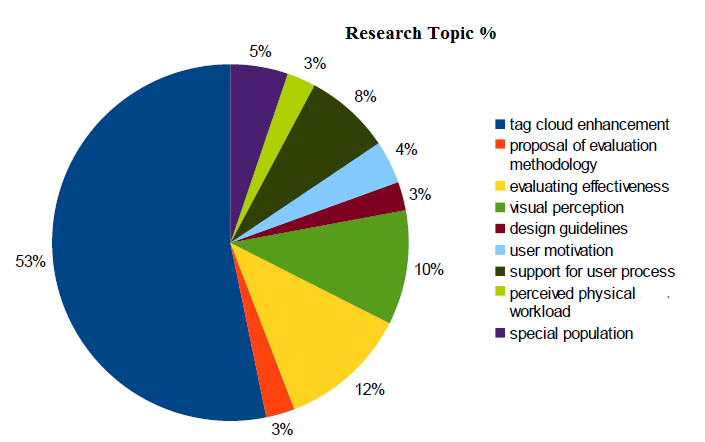
\includegraphics[scale=0.75]{pie1.png}
\caption{\textit{Research topic as a percentage of total papers included in the study}}
\label{fig:pie1}
\end{figure}

\subsection{Research approach and methods}

Table~\vref{tab:evaluation} shows results for research approach and method. By far the most popular methods of evaluation were the `User Performance' and `User Experience' categories, closely followed by `Automated Evaluation of Visualisation' (for brevity these shall be referred to elsewhere as UP, UE and AEV). These three evaluations strategies make up one of the two main categories of evaluation strategies referred to as `visualisation use'. They represent a total of 93 percent of papers surveyed. This is consistent with the findings of \citet{lam12}, where 85 percent of evaluations in information visualisation papers surveyed were representative of these categories. This was thought to be a possible by-product of the traditions in Human Computer Interaction (HCI) and Computer Graphics (GC) which historically have focused on evaluation by controlled experiment, usability and algorithm evaluation. 

All UP category papers reviewed in this study performed controlled experiments, and the vast majority of evaluations within the UE category were carried out via lab questionnaires. 

\begin{table}
\centering
\caption{\textit{Results for the research approach and method}}
\begin{tabular}{|p{2cm}|x{2cm}|p{5cm}|x{2cm}|} \hline
\textbf{Approach}&\textbf{Number}&\textbf{Method}&\textbf{Number}\\ \hline
AEV	&14&algorithm perfomance\par quality metrics&13\par 5\\
UP&32&controlled experiments&32\\
UE&35&informal evaluation\par usability test\par lab questionnaire&3\par3\par30\\
CDA&2&log analysis&2\\
EWP&2&interviews&2\\
VDAR&1&case study&1\\
CTV	&1&field observation\par interviews&1\par1\\
\hline\end{tabular}
\label{tab:evaluation}
\end{table}

\subsection{Visualisation domain}

Visualisation domain category results are found in Table~\vref{tab:domain}. Nearly half of all visualisation domains pertained to the web, with a significant portion of those relating to user generated content \citep[for example][]{bateman08, halvey07, kaser07, skoutas11}. Furthermore, another 11 percent of all domains evaluated visualisations of text corpora. This is understandable given tag cloud visualisation web-based beginnings, and visualisation of label identifiers and textual data is a key advantage of tag clouds. However, it should be possible to apply an information visualisation technique  such as this to any domain where textual data exists. Database search results, particularly for online databases, were another popular domain of research \citep{Wilson11, yamamoto09}.

\begin{table*}
\centering
\caption{\textit{Results for the visualisation domain}}
\begin{tabular}{|l|c|p{5cm}|x{2cm}|} \hline
\textbf{Domain}&\textbf{Number}&\textbf{Sub-domain}&\textbf{Number}\\ \hline
Web&33&user generated content\par database search results\par  recommendation systems&25\par 7 \par 1\\
Mixed media&4&image\par film \par television\par audio&1\par 1\par 1\par 1\\
Text corpora&9&&\\
Mobile phone&2&&\\
Digital forensics&1&&\\
Health and medicine&3&online forums\par tools for the blind&1\par 1\\
Situated displays&1&&\\
Multi-variate data&2&&\\
Database search results&9&online database\par OLAP&7\par 2\\
Geographical information&3&&\\
Situated displays&1&&\\
Software engineering&1&&\\
\hline\end{tabular}
\label{tab:domain}
\end{table*}

\begin{figure}[!htb]
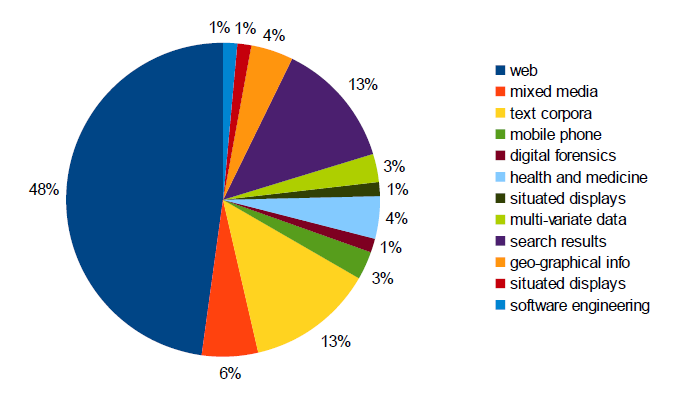
\includegraphics[scale=0.75]{pie2.png}
\caption{\textit{Visualisation domain as a percentage of total papers included in the study}}
\label{fig:pie2}
\end{figure}
